%!TEX output_directory = texaux
%!TEX spellcheck
%!TEX root = ../main.tex

\setlength{\abovedisplayskip}{20pt}
\setlength{\belowdisplayskip}{20pt}

\chapter{Neuronowy model języka}
Wiele mechanizmów przetwarzania języka naturalnego za pomocą sieci neuronowej opiera się na podobnej podstawie. Jest nią probabilistyczny model języka wykorzystujący sieć rekurencyjną do przetwarzania pojawiających się sekwencji (ang. \textit{recurrent neural network language model, RNNLM}). Model ten jest elementem kluczowym w dalszej części pracy, więc poświęcę ten rozdział na jego opis.

%%%%%%%%%%%%%%%%%%%%%%%%%%%%%%%%%%%%%%%%%%%%%%%%%%%%%%%%%%%%%%%%%%%%%%%%%

\section{Modelowanie występowania słów}
Probabilistyczne modelowanie języka polega na określeniu prawdopodobieństw wystąpienia każdego z możliwych słów w danym kontekście. W przypadku \textit{RNNLM} przyjmujemy, że szansa na wystąpienie danego słowa zależy od całej historii. Kontekstem zatem jest dla nas cała sekwencja poprzedzająca dany wyraz. Prowadzi to do następującej zależności:
\[P(w_1^T) = \prod\limits_{t=1}^T P(w_t \mid w_1^{t-1})\]

Zapis $w_i^j$ oznacza podciąg $(w_i, w_{i+1} \dots, w_j)$, $w_1^T$ to pełen ciąg, a $P(w_1 \mid w_1^{t-1})$ jest prawdopodobieństwem wystąpienia słowa $w_1$ bezpośrednio po sekwencji $w_1^{t-1}$. W przypadku $i > j$, $w_i^j$ jest ciągiem pustym.

%%%%%%%%%%%%%%%%%%%%%%%%%%%%%%%%%%%%%%%%%%%%%%%%%%%%%%%%%%%%%%%%%%%%%%%%%

\section{Architektura sieci}
\textit{RNNLM} składa się z tzw. warstwy zanurzeń, po której następuje warstwa rekurencyjna, a całość kończy się \textit{softmaxem} produkującym prawdopodobieństwa warunkowe, o których była mowa w poprzedniej sekcji. Warstwa zanurzeń (ang. \textit{embedding layer}) odpowiada za przekształcenie sekwencji słów na format liczbowy. Sekcja~\ref{wektory} zawiera więcej informacji na ten temat. Na razie wystarczy, że wejściowa sekwencja słów jest przekształcana na ciąg wektorów, który może być przetwarzany przez sieć rekurencyjną.

Niech $V = \lbrace v_1, v_2, \dots, v_{|V|} \rbrace$ oznacza słownik, czyli zbiór wszystkich słów występujących w języku. Wejściem do sieci jest ciąg $w_1^T$, składający się ze słów. Wygodnie jest o nim myśleć jako o ciągu indeksów, tzn. sekwencja w języku naturalnym to $(v_{w_1}, \dots, v_{w_T})$. Kolejne kroki \textit{RNNLM} wyglądają tak:
\begin{enumerate}
    \item \textbf{Zanurzenia}: ciąg $w_1^T$ jest przetwarzany na $x_1^T$ -- ciąg wektorów w $\mathbb{R}^n$.
    \item \textbf{\textit{RNN}}: sieć rekurencyjna czyta $x_1^T$ produkując $h_1^T$, gdzie $h_i$ jest wynikiem przejścia po $x_1^i$, a $h_0 = \vv{0}$.
    \item \textbf{Softmax}: dla każdego $i \in \{0,\dots,T-1\}$ wektor $h_i$ wchodzi do warstwy \textit{softmax}, która najpierw przekształceniem afinicznym wkłada go w $\mathbb{R}^{|V|}$, a następnie funkcją \textit{softmax} przerabia na wektor prawdopodobieństw $p_{i+1}$. W ten sposób powstaje ciąg $p_1^T$, którego każdy element jest pewnym rozkładem prawdopodobieństwa na $V$.
\end{enumerate}

\begin{figure}[H]
  \centering
    \hspace*{2cm}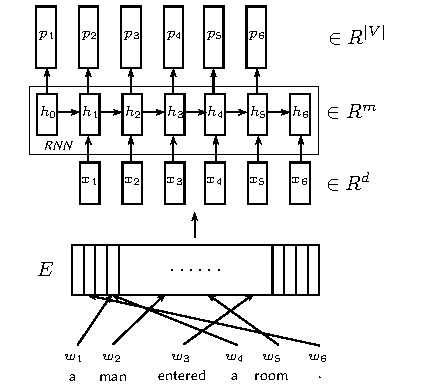
\includegraphics[width=0.9\textwidth]{chapter2/img/rnnlm.eps}
  \caption{\small{Schemat przetwarzania pojedynczej sekwencji przez \textit{RNNLM}. Zamiana słów na wektory odbywa się przez indeksowanie macierzy $E$, $m$ jest rozmiarem stanu \textit{RNN}, a~$d$~rozmiarem zanurzenia.}}
\end{figure}

%%%%%%%%%%%%%%%%%%%%%%%%%%%%%%%%%%%%%%%%%%%%%%%%%%%%%%%%%%%%%%%%%%%%%%%%%

\section{Proces uczenia}
Elementy wynikowego ciągu $p_1^T$ możemy interpretować jako warunkowe rozkłady prawdopodobieństwa na kolejnych pozycjach $w_1^T$. Na przykład $p_3$ określa prawdopodobieństwa poszczególnych słów z $V$ po sekwencji $w_1^2$. Wiemy, że naprawdę pojawiło się tam słowo $w_3$. Według modelu szansa takiego zjawiska to $(p_3)_{w_3}$, czyli element wektora $p_3$ znajdujący się na pozycji $w_3$.

Uczenie neuronowego modelu języka polega na maksymalizowaniu prawdopodobieństw wystąpienia sekwencji, które model faktycznie widzi, czyli tych, co do których zakładamy, że są poprawne. Inaczej mówiąc maksymalizujemy wiarygodność zbioru uczącego. Na podstawie $p_1^T$ możemy obliczyć prawdopodobieństwo zaistnienia całego ciągu. Niech $\theta$ oznacza parametry modelu.
\[\hat{P}(w_1^T\, ;\, \theta) = \prod\limits_{t=1}^T \hat{P}(w_t \mid w_1^{t-1}\, ;\, \theta ) = \prod\limits_{t=1}^T {(p_t)}_{w_t}\]

W praktyce długie iloczyny nie sprawdzają się dobrze ze względu na ograniczenia numeryczne. Chcąc znaleźć parametry maksymalizujące $\hat{P}(w_1^T)$ wystarczy jednak wyznaczyć takie, które maksymalizują $\ln(\hat{P}(w_1^T))$. W uczeniu maszynowym panuje konwencja, według której zwykle minimalizujemy koszt, więc ostateczna forma
optymalizowanej wartości to
\[-\sum\limits_{t=1}^T \ln((p_t)_{w_t}).\]

Jest to bardzo popularna funkcja kosztu, wywodząca się z metody największej wiarygodności. W literaturze nosi nazwę \textit{negative log likelihood}, czasami skracane do \textit{nll}.

%%%%%%%%%%%%%%%%%%%%%%%%%%%%%%%%%%%%%%%%%%%%%%%%%%%%%%%%%%%%%%%%%%%%%%%%%

\section{Reprezentacje wektorowe} \label{wektory}
Większość metod uczenia maszynowego, w tym sieci neuronowe, pracuje na liczbach. Zanim będziemy mogli wprowadzić do algorytmu sekwencje w języku naturalnym, musimy wyznaczyć dla nich odpowiednie liczbowe reprezentacje. Najprostszym pomysłem na przedstawienie słów jako wektorów jest użycie przestrzeni $\mathbb{R}^{|V|}$, w której każde słowo jest kodowane binarnie jako wektor o jednej współrzędnej niezerowej. W ten sposób powstają tzw. rzadkie reprezentacje słów:
\[
\begin{aligned}
    \mathrm{vec_{sparse}}(v_i) &=
    \begin{bmatrix}
        0 \\
        \vdots \\
        0 \\
        1 \\
        0 \\
        \vdots \\
        0
    \end{bmatrix}
\end{aligned} \leftarrow i\text{-ta współrzędna}
\]

Rzadkie wektory mają kilka problemów. Po pierwsze, nie niosą żadnej istotnej informacji o słowach. Jedyna cecha, którą oddają, to kolejność słów w słowniku, co do której i tak nie przyjmujemy żadnych założeń; może być przypadkowa. Po drugie, są bardzo nieefektywne. Używamy tylko jednej współrzędnej, a wymiar może być bardzo duży; słownik może liczyć dziesiątki, a nawet setki tysięcy słów. Ten fakt ma dalsze konsekwencje: macierz $W$ czytającej sekwencje sieci rekurencyjnej musi być bardzo duża.

Rozwiązaniem tych kłopotów jest skorzystanie z gęstych reprezentacji słów, których sieć uczy się jednocześnie z pozostałymi parametrami. Warstwa zanurzeń jest sparametryzowana przez macierz $E \in \mathbb{R}^{d \times |V|}$ o kolumnach $E_1, E_2, \dots, E_{|V|}$, gdzie $d$ jest wybranym rozmiarem zanurzenia. Gęsty wektor dla słowa otrzymujemy mnożąc $E$ przez wektor rzadki, co sprowadza się do wyboru odpowiedniej kolumny:
\[\mathrm{vec_{dense}}(v_i) = E \cdot \mathrm{vec_{sparse}}(v_i) = E_i\]

Podczas minimalizowania kosztu sieć sama będzie szukała optymalnych reprezentacji. Oczekujemy, że dla słów pojawiających się w podobnych kontekstach wyuczone wektory będą podobne. To z kolei powinno spowodować, że prawdopodobieństwa ich wystąpień również okażą się zbliżone.

Okazuje się, że faktycznie tak jest. Otrzymane w ten sposób reprezentacje słów zawierają istotne informacje semantyczne. Podobne słowa dostają bliskie wektory, a~wymiar przestrzeni zanurzeń zostaje znacznie zredukowany (w praktyce najczęściej spotyka się $100 \leq d \leq 300$). Gęste reprezentacje słów okazały się na tyle przydatne, że powstały wyspecjalizowane architektury przeznaczone do ich obliczania. Do najpopularniejszych z nich należą Word2Vec \cite{w2v} i GloVe \cite{glove}.

Jakość otrzymanych wektorów mocno zależy od jakości danych uczących. Małe próbki języka nie dadzą wystarczającej informacji o statystycznym występowaniu słów w kontekstach. Wyuczenie bardzo dobrych zanurzeń słów wymaga zatem dużego zbioru tekstów, a co za tym idzie, pewnego nakładu czasu. Z tego powodu na początkową wartość macierzy $E$ często wybiera się wstępnie obliczone wektory. Skraca to czas potrzebny na znalezienie reprezentacji oraz zmniejsza potrzebną do nauczenia sieci ilość danych. Uczenie zanurzeń zaczynając od takiego ich zainicjowania zwykle pozwala poprawić jakość modelu. Często poprawa jest jednak na tyle mała, że lepiej zaoszczędzić na czasie i potraktować je jako stałe.

Wektory dla języka angielskiego obliczone przez Word2Vec i GloVe są publicznie dostępne. Wykorzystane zbiory danych to odpowiednio korpus Google News, liczący około 100 miliardów słów, i Common Crawl (840 miliardów słów).

Pomysł wykorzystania gęstych wektorów do reprezentowania słów pojawił się po raz pierwszy w \cite{bengiolm}. Tam też został opisany neuronowy model języka, chociaż w odrobinę prostszej wersji: kontekst był obcinany do kilku poprzedzających słów. Architektura wykorzystująca sieci rekurencyjne i nieograniczony kontekst pojawiła się w \cite{rnnlm}.

%%%%%%%%%%%%%%%%%%%%%%%%%%%%%%%%%%%%%%%%%%%%%%%%%%%%%%%%%%%%%%%%%%%%%%%%%

\section{Generowanie tekstu}\label{gen}
Po znalezieniu optymalnych parametrów $\theta_{opt}$ możliwe jest próbkowanie powstałego rozkładu prawdopodobieństwa w celu generowania nowych tekstów. Zwykle podczas uczenia wprowadza się sztuczne słowo $\mathbf{start}$ oznaczające początek sekwencji. Przyjmujemy, że każda poprawna sekwencja rozpoczyna się od $\mathbf{start}$. Zaczynamy więc od ciągu jednoelementowego $w_1^1$, gdzie $w_1 = \mathbf{start}$. Najprostszy generator w~każdym kroku wybiera najbardziej prawdopodobne słowo. Dla $i>1$:
\[w_i = \argmax\limits_{v \in V} \hat{P}(v \mid w_1^{i-1}\, ;\, \theta_{opt})\]

Analogicznie do słowa $\mathbf{start}$ wzbogacamy dane o słowo $\mathbf{end}$, oznaczające koniec sekwencji. Generator kończy pracę, kiedy ostatnim wybranym słowem jest $\mathbf{end}$.

Powyższa metoda tworzy \textit{ciąg najbardziej prawdopodobnych} słów. Naprawdę jednak zależy nam na \textit{najbardziej prawdopodobnym ciągu} słów. Wyobraźmy sobie hipotetyczną sytuację, w której
\[\hat{P}(\text{\textit{the}} \mid (\mathbf{start})\, ;\, \theta_{opt}) > \hat{P}(\text{\textit{no}} \mid (\mathbf{start})\, ;\, \theta_{opt}),\]
pomimo tego, że zdanie \textit{no, thanks.} jest bardziej prawdopodobne od dowolnego zdania rozpoczynającego się od \textit{the}. Nie chcemy wtedy w~pierwszym kroku zachłannie decydować się na \textit{the}.

W przypadku języka naturalnego zbadanie prawdopodobieństwa wszystkich możliwych sekwencji jest oczywiście niewykonalne. Nawet niewielki słowniku rzędu 10 tysięcy słów pozwala na $10^{20}$ możliwości ułożenia pięciowyrazowego zdania. Konieczność sprawdzenia tylu przypadków wyklucza wszelkie praktyczne zastosowania, dlatego potrzebujemy jakiejś heurystyki zawężającej przestrzeń poszukiwań do akceptowalnych rozmiarów. Popularnym sposobem osiągnięcia tego celu jest przeszukiwanie wiązkowe (ang. \textit{beam search}).

%%%%%%%%%%%%%%%%%%%

\subsection{Przeszukiwanie wiązkowe} \label{beamsearch}
Wędrując po drzewie możliwości w algorytmie \textit{beam search} w każdym momencie pamiętamy tylko $K$ najlepszych napotkanych ścieżek. Liczba $K$ jest parametrem algorytmu i ma duży wpływ na jego wydajność i zachowanie. Odwiedzając dany liść rozpatrujemy wszystkich jego sąsiadów (w przypadku generowania tekstu zawsze jest to $|V|$). W ten sposób dla wiązki rozmiaru $K$ dostajemy $K \cdot |V|$ możliwych kontynuacji, spośród których wybieramy $K$ najlepszych. Sekwencje kończące się symbolem $\mathbf{end}$ są uznawane za zakończone. Zostają w wiązce dopóki nie zostaną wyparte przez coś lepszego, ale nie są dalej rozwijane. Rozpoczynamy od jednoelementowego ciągu $(\mathbf{start})$, po czym tworzymy początkową wiązkę $K$ najbardziej prawdopodobnych słów. Symbol $^\frown$ w pseudokodzie algorytmu oznacza konkatenację ciągów.

\begin{algorithm}[h]
    \SetAlgorithmName{Algorytm}
    \\\\$K$ -- szerokość wiązki\\[5pt]
    $beam \gets \{((\mathbf{start}), 0)\}$, początkowy zbiór par $(sekwencja, wynik)$\\
    \While{\textnormal{istnieją niezakończone ciągi w} $beam$}{
        $cont \gets \{\}$\\
        \For{$(seq,\ scr) \mathbf{\ in\ } beam$}{
            \For{$v \mathbf{\ in\ } V$}{
                $p_{log} \gets \ln(\hat{P}(v \mid seq\, ;\, \theta_{opt}))$\\
                $cont \gets cont \cup \{(seq^\frown (v),\ scr + p_{log})\}$
            }
        }
        $beam \gets$ podzbiór $K$ elementów $cont$ o najwyższych wynikach
    }
    \Return element $beam$ o najwyższym wyniku
    \caption{Przeszukiwanie wiązkowe}
\end{algorithm}

Warto zauważyć, że ta metoda cały czas jest deterministyczna. Dany zestaw parametrów sieci zawsze wyprodukuje ten sam tekst. Powyższy generator można na różne sposoby modyfikować. Więcej na ten temat w następnym rozdziale.

\begin{figure}[H]
  \centering
    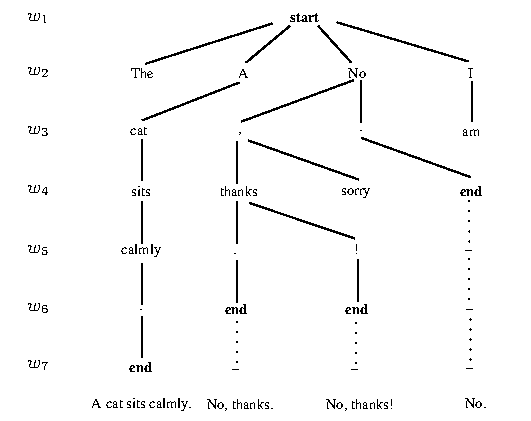
\includegraphics[width=\textwidth]{chapter2/img/bs.eps}
  \caption{\small{Hipotetyczny przykład działania algorytmu \textit{beam search} dla wiązki o rozmiarze 4. Dla przejrzystości w każdym kroku zaznaczono tylko elementy zawarte w wiązce.}}
\end{figure}
